% Created by tikzDevice version 0.12.6 on 2025-02-14 03:21:02
% !TEX encoding = UTF-8 Unicode
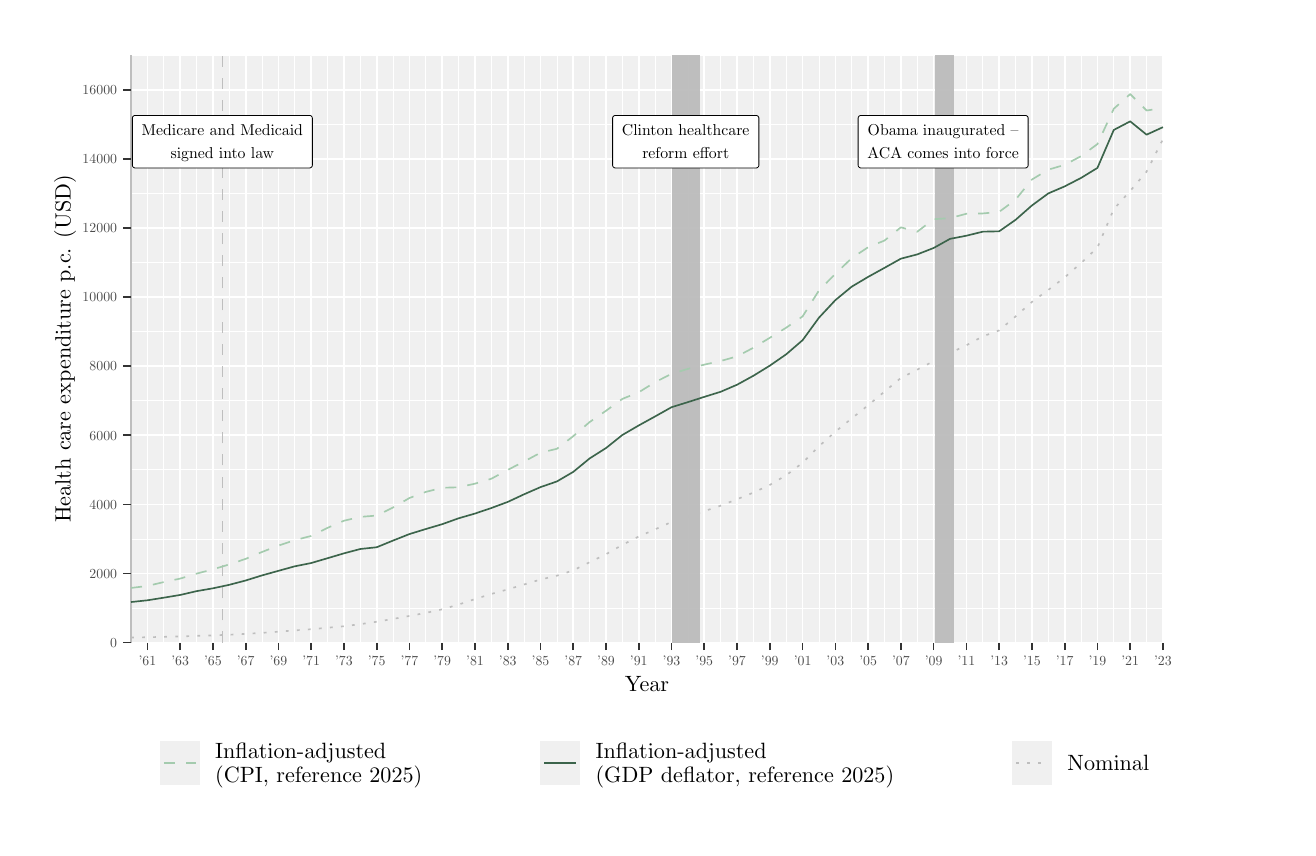
\begin{tikzpicture}[x=1pt,y=1pt]
\definecolor{fillColor}{RGB}{255,255,255}
\path[use as bounding box,fill=fillColor,fill opacity=0.00] (0,0) rectangle (455.30,289.08);
\begin{scope}
\path[clip] (  0.00,  0.00) rectangle (455.30,289.08);
\definecolor{drawColor}{RGB}{255,255,255}
\definecolor{fillColor}{RGB}{255,255,255}

\path[draw=drawColor,line width= 0.6pt,line join=round,line cap=round,fill=fillColor] ( -0.00,  0.00) rectangle (455.30,289.08);
\end{scope}
\begin{scope}
\path[clip] (  0.00,  0.00) rectangle (455.30,289.08);
\definecolor{fillColor}{gray}{0.94}

\path[fill=fillColor] ( 37.26, 66.89) rectangle (410.30,279.08);
\definecolor{drawColor}{RGB}{255,255,255}

\path[draw=drawColor,line width= 0.3pt,line join=round] ( 37.26, 79.37) --
	(410.30, 79.37);

\path[draw=drawColor,line width= 0.3pt,line join=round] ( 37.26,104.33) --
	(410.30,104.33);

\path[draw=drawColor,line width= 0.3pt,line join=round] ( 37.26,129.30) --
	(410.30,129.30);

\path[draw=drawColor,line width= 0.3pt,line join=round] ( 37.26,154.26) --
	(410.30,154.26);

\path[draw=drawColor,line width= 0.3pt,line join=round] ( 37.26,179.22) --
	(410.30,179.22);

\path[draw=drawColor,line width= 0.3pt,line join=round] ( 37.26,204.19) --
	(410.30,204.19);

\path[draw=drawColor,line width= 0.3pt,line join=round] ( 37.26,229.15) --
	(410.30,229.15);

\path[draw=drawColor,line width= 0.3pt,line join=round] ( 37.26,254.12) --
	(410.30,254.12);

\path[draw=drawColor,line width= 0.3pt,line join=round] ( 37.26,279.08) --
	(410.30,279.08);

\path[draw=drawColor,line width= 0.3pt,line join=round] ( 37.35, 66.89) --
	( 37.35,279.08);

\path[draw=drawColor,line width= 0.3pt,line join=round] ( 49.19, 66.89) --
	( 49.19,279.08);

\path[draw=drawColor,line width= 0.3pt,line join=round] ( 61.03, 66.89) --
	( 61.03,279.08);

\path[draw=drawColor,line width= 0.3pt,line join=round] ( 72.86, 66.89) --
	( 72.86,279.08);

\path[draw=drawColor,line width= 0.3pt,line join=round] ( 84.70, 66.89) --
	( 84.70,279.08);

\path[draw=drawColor,line width= 0.3pt,line join=round] ( 96.54, 66.89) --
	( 96.54,279.08);

\path[draw=drawColor,line width= 0.3pt,line join=round] (108.37, 66.89) --
	(108.37,279.08);

\path[draw=drawColor,line width= 0.3pt,line join=round] (120.21, 66.89) --
	(120.21,279.08);

\path[draw=drawColor,line width= 0.3pt,line join=round] (132.05, 66.89) --
	(132.05,279.08);

\path[draw=drawColor,line width= 0.3pt,line join=round] (143.89, 66.89) --
	(143.89,279.08);

\path[draw=drawColor,line width= 0.3pt,line join=round] (155.72, 66.89) --
	(155.72,279.08);

\path[draw=drawColor,line width= 0.3pt,line join=round] (167.56, 66.89) --
	(167.56,279.08);

\path[draw=drawColor,line width= 0.3pt,line join=round] (179.40, 66.89) --
	(179.40,279.08);

\path[draw=drawColor,line width= 0.3pt,line join=round] (191.24, 66.89) --
	(191.24,279.08);

\path[draw=drawColor,line width= 0.3pt,line join=round] (203.07, 66.89) --
	(203.07,279.08);

\path[draw=drawColor,line width= 0.3pt,line join=round] (214.91, 66.89) --
	(214.91,279.08);

\path[draw=drawColor,line width= 0.3pt,line join=round] (226.75, 66.89) --
	(226.75,279.08);

\path[draw=drawColor,line width= 0.3pt,line join=round] (238.58, 66.89) --
	(238.58,279.08);

\path[draw=drawColor,line width= 0.3pt,line join=round] (250.42, 66.89) --
	(250.42,279.08);

\path[draw=drawColor,line width= 0.3pt,line join=round] (262.26, 66.89) --
	(262.26,279.08);

\path[draw=drawColor,line width= 0.3pt,line join=round] (274.10, 66.89) --
	(274.10,279.08);

\path[draw=drawColor,line width= 0.3pt,line join=round] (285.93, 66.89) --
	(285.93,279.08);

\path[draw=drawColor,line width= 0.3pt,line join=round] (297.77, 66.89) --
	(297.77,279.08);

\path[draw=drawColor,line width= 0.3pt,line join=round] (309.61, 66.89) --
	(309.61,279.08);

\path[draw=drawColor,line width= 0.3pt,line join=round] (321.44, 66.89) --
	(321.44,279.08);

\path[draw=drawColor,line width= 0.3pt,line join=round] (333.28, 66.89) --
	(333.28,279.08);

\path[draw=drawColor,line width= 0.3pt,line join=round] (345.12, 66.89) --
	(345.12,279.08);

\path[draw=drawColor,line width= 0.3pt,line join=round] (356.96, 66.89) --
	(356.96,279.08);

\path[draw=drawColor,line width= 0.3pt,line join=round] (368.79, 66.89) --
	(368.79,279.08);

\path[draw=drawColor,line width= 0.3pt,line join=round] (380.63, 66.89) --
	(380.63,279.08);

\path[draw=drawColor,line width= 0.3pt,line join=round] (392.47, 66.89) --
	(392.47,279.08);

\path[draw=drawColor,line width= 0.3pt,line join=round] (404.31, 66.89) --
	(404.31,279.08);

\path[draw=drawColor,line width= 0.6pt,line join=round] ( 37.26, 66.89) --
	(410.30, 66.89);

\path[draw=drawColor,line width= 0.6pt,line join=round] ( 37.26, 91.85) --
	(410.30, 91.85);

\path[draw=drawColor,line width= 0.6pt,line join=round] ( 37.26,116.81) --
	(410.30,116.81);

\path[draw=drawColor,line width= 0.6pt,line join=round] ( 37.26,141.78) --
	(410.30,141.78);

\path[draw=drawColor,line width= 0.6pt,line join=round] ( 37.26,166.74) --
	(410.30,166.74);

\path[draw=drawColor,line width= 0.6pt,line join=round] ( 37.26,191.71) --
	(410.30,191.71);

\path[draw=drawColor,line width= 0.6pt,line join=round] ( 37.26,216.67) --
	(410.30,216.67);

\path[draw=drawColor,line width= 0.6pt,line join=round] ( 37.26,241.63) --
	(410.30,241.63);

\path[draw=drawColor,line width= 0.6pt,line join=round] ( 37.26,266.60) --
	(410.30,266.60);

\path[draw=drawColor,line width= 0.6pt,line join=round] ( 43.27, 66.89) --
	( 43.27,279.08);

\path[draw=drawColor,line width= 0.6pt,line join=round] ( 55.10, 66.89) --
	( 55.10,279.08);

\path[draw=drawColor,line width= 0.6pt,line join=round] ( 66.95, 66.89) --
	( 66.95,279.08);

\path[draw=drawColor,line width= 0.6pt,line join=round] ( 78.78, 66.89) --
	( 78.78,279.08);

\path[draw=drawColor,line width= 0.6pt,line join=round] ( 90.62, 66.89) --
	( 90.62,279.08);

\path[draw=drawColor,line width= 0.6pt,line join=round] (102.45, 66.89) --
	(102.45,279.08);

\path[draw=drawColor,line width= 0.6pt,line join=round] (114.30, 66.89) --
	(114.30,279.08);

\path[draw=drawColor,line width= 0.6pt,line join=round] (126.13, 66.89) --
	(126.13,279.08);

\path[draw=drawColor,line width= 0.6pt,line join=round] (137.97, 66.89) --
	(137.97,279.08);

\path[draw=drawColor,line width= 0.6pt,line join=round] (149.80, 66.89) --
	(149.80,279.08);

\path[draw=drawColor,line width= 0.6pt,line join=round] (161.65, 66.89) --
	(161.65,279.08);

\path[draw=drawColor,line width= 0.6pt,line join=round] (173.48, 66.89) --
	(173.48,279.08);

\path[draw=drawColor,line width= 0.6pt,line join=round] (185.32, 66.89) --
	(185.32,279.08);

\path[draw=drawColor,line width= 0.6pt,line join=round] (197.15, 66.89) --
	(197.15,279.08);

\path[draw=drawColor,line width= 0.6pt,line join=round] (209.00, 66.89) --
	(209.00,279.08);

\path[draw=drawColor,line width= 0.6pt,line join=round] (220.82, 66.89) --
	(220.82,279.08);

\path[draw=drawColor,line width= 0.6pt,line join=round] (232.67, 66.89) --
	(232.67,279.08);

\path[draw=drawColor,line width= 0.6pt,line join=round] (244.50, 66.89) --
	(244.50,279.08);

\path[draw=drawColor,line width= 0.6pt,line join=round] (256.34, 66.89) --
	(256.34,279.08);

\path[draw=drawColor,line width= 0.6pt,line join=round] (268.17, 66.89) --
	(268.17,279.08);

\path[draw=drawColor,line width= 0.6pt,line join=round] (280.02, 66.89) --
	(280.02,279.08);

\path[draw=drawColor,line width= 0.6pt,line join=round] (291.85, 66.89) --
	(291.85,279.08);

\path[draw=drawColor,line width= 0.6pt,line join=round] (303.69, 66.89) --
	(303.69,279.08);

\path[draw=drawColor,line width= 0.6pt,line join=round] (315.52, 66.89) --
	(315.52,279.08);

\path[draw=drawColor,line width= 0.6pt,line join=round] (327.37, 66.89) --
	(327.37,279.08);

\path[draw=drawColor,line width= 0.6pt,line join=round] (339.20, 66.89) --
	(339.20,279.08);

\path[draw=drawColor,line width= 0.6pt,line join=round] (351.04, 66.89) --
	(351.04,279.08);

\path[draw=drawColor,line width= 0.6pt,line join=round] (362.87, 66.89) --
	(362.87,279.08);

\path[draw=drawColor,line width= 0.6pt,line join=round] (374.72, 66.89) --
	(374.72,279.08);

\path[draw=drawColor,line width= 0.6pt,line join=round] (386.55, 66.89) --
	(386.55,279.08);

\path[draw=drawColor,line width= 0.6pt,line join=round] (398.39, 66.89) --
	(398.39,279.08);

\path[draw=drawColor,line width= 0.6pt,line join=round] (410.22, 66.89) --
	(410.22,279.08);
\definecolor{drawColor}{RGB}{190,190,190}

\path[draw=drawColor,line width= 0.6pt,line join=round] ( 37.34, 66.89) -- ( 37.34,279.08);
\definecolor{fillColor}{RGB}{190,190,190}

\path[fill=fillColor,fill opacity=0.01] (232.67, 66.89) rectangle (242.93,279.08);

\path[fill=fillColor,fill opacity=0.01] (232.67, 66.89) rectangle (242.93,279.08);

\path[fill=fillColor,fill opacity=0.01] (232.67, 66.89) rectangle (242.93,279.08);

\path[fill=fillColor,fill opacity=0.01] (232.67, 66.89) rectangle (242.93,279.08);

\path[fill=fillColor,fill opacity=0.01] (232.67, 66.89) rectangle (242.93,279.08);

\path[fill=fillColor,fill opacity=0.01] (232.67, 66.89) rectangle (242.93,279.08);

\path[fill=fillColor,fill opacity=0.01] (232.67, 66.89) rectangle (242.93,279.08);

\path[fill=fillColor,fill opacity=0.01] (232.67, 66.89) rectangle (242.93,279.08);

\path[fill=fillColor,fill opacity=0.01] (232.67, 66.89) rectangle (242.93,279.08);

\path[fill=fillColor,fill opacity=0.01] (232.67, 66.89) rectangle (242.93,279.08);

\path[fill=fillColor,fill opacity=0.01] (232.67, 66.89) rectangle (242.93,279.08);

\path[fill=fillColor,fill opacity=0.01] (232.67, 66.89) rectangle (242.93,279.08);

\path[fill=fillColor,fill opacity=0.01] (232.67, 66.89) rectangle (242.93,279.08);

\path[fill=fillColor,fill opacity=0.01] (232.67, 66.89) rectangle (242.93,279.08);

\path[fill=fillColor,fill opacity=0.01] (232.67, 66.89) rectangle (242.93,279.08);

\path[fill=fillColor,fill opacity=0.01] (232.67, 66.89) rectangle (242.93,279.08);

\path[fill=fillColor,fill opacity=0.01] (232.67, 66.89) rectangle (242.93,279.08);

\path[fill=fillColor,fill opacity=0.01] (232.67, 66.89) rectangle (242.93,279.08);

\path[fill=fillColor,fill opacity=0.01] (232.67, 66.89) rectangle (242.93,279.08);

\path[fill=fillColor,fill opacity=0.01] (232.67, 66.89) rectangle (242.93,279.08);

\path[fill=fillColor,fill opacity=0.01] (232.67, 66.89) rectangle (242.93,279.08);

\path[fill=fillColor,fill opacity=0.01] (232.67, 66.89) rectangle (242.93,279.08);

\path[fill=fillColor,fill opacity=0.01] (232.67, 66.89) rectangle (242.93,279.08);

\path[fill=fillColor,fill opacity=0.01] (232.67, 66.89) rectangle (242.93,279.08);

\path[fill=fillColor,fill opacity=0.01] (232.67, 66.89) rectangle (242.93,279.08);

\path[fill=fillColor,fill opacity=0.01] (232.67, 66.89) rectangle (242.93,279.08);

\path[fill=fillColor,fill opacity=0.01] (232.67, 66.89) rectangle (242.93,279.08);

\path[fill=fillColor,fill opacity=0.01] (232.67, 66.89) rectangle (242.93,279.08);

\path[fill=fillColor,fill opacity=0.01] (232.67, 66.89) rectangle (242.93,279.08);

\path[fill=fillColor,fill opacity=0.01] (232.67, 66.89) rectangle (242.93,279.08);

\path[fill=fillColor,fill opacity=0.01] (232.67, 66.89) rectangle (242.93,279.08);

\path[fill=fillColor,fill opacity=0.01] (232.67, 66.89) rectangle (242.93,279.08);

\path[fill=fillColor,fill opacity=0.01] (232.67, 66.89) rectangle (242.93,279.08);

\path[fill=fillColor,fill opacity=0.01] (232.67, 66.89) rectangle (242.93,279.08);

\path[fill=fillColor,fill opacity=0.01] (232.67, 66.89) rectangle (242.93,279.08);

\path[fill=fillColor,fill opacity=0.01] (232.67, 66.89) rectangle (242.93,279.08);

\path[fill=fillColor,fill opacity=0.01] (232.67, 66.89) rectangle (242.93,279.08);

\path[fill=fillColor,fill opacity=0.01] (232.67, 66.89) rectangle (242.93,279.08);

\path[fill=fillColor,fill opacity=0.01] (232.67, 66.89) rectangle (242.93,279.08);

\path[fill=fillColor,fill opacity=0.01] (232.67, 66.89) rectangle (242.93,279.08);

\path[fill=fillColor,fill opacity=0.01] (232.67, 66.89) rectangle (242.93,279.08);

\path[fill=fillColor,fill opacity=0.01] (232.67, 66.89) rectangle (242.93,279.08);

\path[fill=fillColor,fill opacity=0.01] (232.67, 66.89) rectangle (242.93,279.08);

\path[fill=fillColor,fill opacity=0.01] (232.67, 66.89) rectangle (242.93,279.08);

\path[fill=fillColor,fill opacity=0.01] (232.67, 66.89) rectangle (242.93,279.08);

\path[fill=fillColor,fill opacity=0.01] (232.67, 66.89) rectangle (242.93,279.08);

\path[fill=fillColor,fill opacity=0.01] (232.67, 66.89) rectangle (242.93,279.08);

\path[fill=fillColor,fill opacity=0.01] (232.67, 66.89) rectangle (242.93,279.08);

\path[fill=fillColor,fill opacity=0.01] (232.67, 66.89) rectangle (242.93,279.08);

\path[fill=fillColor,fill opacity=0.01] (232.67, 66.89) rectangle (242.93,279.08);

\path[fill=fillColor,fill opacity=0.01] (232.67, 66.89) rectangle (242.93,279.08);

\path[fill=fillColor,fill opacity=0.01] (232.67, 66.89) rectangle (242.93,279.08);

\path[fill=fillColor,fill opacity=0.01] (232.67, 66.89) rectangle (242.93,279.08);

\path[fill=fillColor,fill opacity=0.01] (232.67, 66.89) rectangle (242.93,279.08);

\path[fill=fillColor,fill opacity=0.01] (232.67, 66.89) rectangle (242.93,279.08);

\path[fill=fillColor,fill opacity=0.01] (232.67, 66.89) rectangle (242.93,279.08);

\path[fill=fillColor,fill opacity=0.01] (232.67, 66.89) rectangle (242.93,279.08);

\path[fill=fillColor,fill opacity=0.01] (232.67, 66.89) rectangle (242.93,279.08);

\path[fill=fillColor,fill opacity=0.01] (232.67, 66.89) rectangle (242.93,279.08);

\path[fill=fillColor,fill opacity=0.01] (232.67, 66.89) rectangle (242.93,279.08);

\path[fill=fillColor,fill opacity=0.01] (232.67, 66.89) rectangle (242.93,279.08);

\path[fill=fillColor,fill opacity=0.01] (232.67, 66.89) rectangle (242.93,279.08);

\path[fill=fillColor,fill opacity=0.01] (232.67, 66.89) rectangle (242.93,279.08);

\path[fill=fillColor,fill opacity=0.01] (232.67, 66.89) rectangle (242.93,279.08);

\path[fill=fillColor,fill opacity=0.01] (327.68, 66.89) rectangle (334.59,279.08);

\path[fill=fillColor,fill opacity=0.01] (327.68, 66.89) rectangle (334.59,279.08);

\path[fill=fillColor,fill opacity=0.01] (327.68, 66.89) rectangle (334.59,279.08);

\path[fill=fillColor,fill opacity=0.01] (327.68, 66.89) rectangle (334.59,279.08);

\path[fill=fillColor,fill opacity=0.01] (327.68, 66.89) rectangle (334.59,279.08);

\path[fill=fillColor,fill opacity=0.01] (327.68, 66.89) rectangle (334.59,279.08);

\path[fill=fillColor,fill opacity=0.01] (327.68, 66.89) rectangle (334.59,279.08);

\path[fill=fillColor,fill opacity=0.01] (327.68, 66.89) rectangle (334.59,279.08);

\path[fill=fillColor,fill opacity=0.01] (327.68, 66.89) rectangle (334.59,279.08);

\path[fill=fillColor,fill opacity=0.01] (327.68, 66.89) rectangle (334.59,279.08);

\path[fill=fillColor,fill opacity=0.01] (327.68, 66.89) rectangle (334.59,279.08);

\path[fill=fillColor,fill opacity=0.01] (327.68, 66.89) rectangle (334.59,279.08);

\path[fill=fillColor,fill opacity=0.01] (327.68, 66.89) rectangle (334.59,279.08);

\path[fill=fillColor,fill opacity=0.01] (327.68, 66.89) rectangle (334.59,279.08);

\path[fill=fillColor,fill opacity=0.01] (327.68, 66.89) rectangle (334.59,279.08);

\path[fill=fillColor,fill opacity=0.01] (327.68, 66.89) rectangle (334.59,279.08);

\path[fill=fillColor,fill opacity=0.01] (327.68, 66.89) rectangle (334.59,279.08);

\path[fill=fillColor,fill opacity=0.01] (327.68, 66.89) rectangle (334.59,279.08);

\path[fill=fillColor,fill opacity=0.01] (327.68, 66.89) rectangle (334.59,279.08);

\path[fill=fillColor,fill opacity=0.01] (327.68, 66.89) rectangle (334.59,279.08);

\path[fill=fillColor,fill opacity=0.01] (327.68, 66.89) rectangle (334.59,279.08);

\path[fill=fillColor,fill opacity=0.01] (327.68, 66.89) rectangle (334.59,279.08);

\path[fill=fillColor,fill opacity=0.01] (327.68, 66.89) rectangle (334.59,279.08);

\path[fill=fillColor,fill opacity=0.01] (327.68, 66.89) rectangle (334.59,279.08);

\path[fill=fillColor,fill opacity=0.01] (327.68, 66.89) rectangle (334.59,279.08);

\path[fill=fillColor,fill opacity=0.01] (327.68, 66.89) rectangle (334.59,279.08);

\path[fill=fillColor,fill opacity=0.01] (327.68, 66.89) rectangle (334.59,279.08);

\path[fill=fillColor,fill opacity=0.01] (327.68, 66.89) rectangle (334.59,279.08);

\path[fill=fillColor,fill opacity=0.01] (327.68, 66.89) rectangle (334.59,279.08);

\path[fill=fillColor,fill opacity=0.01] (327.68, 66.89) rectangle (334.59,279.08);

\path[fill=fillColor,fill opacity=0.01] (327.68, 66.89) rectangle (334.59,279.08);

\path[fill=fillColor,fill opacity=0.01] (327.68, 66.89) rectangle (334.59,279.08);

\path[fill=fillColor,fill opacity=0.01] (327.68, 66.89) rectangle (334.59,279.08);

\path[fill=fillColor,fill opacity=0.01] (327.68, 66.89) rectangle (334.59,279.08);

\path[fill=fillColor,fill opacity=0.01] (327.68, 66.89) rectangle (334.59,279.08);

\path[fill=fillColor,fill opacity=0.01] (327.68, 66.89) rectangle (334.59,279.08);

\path[fill=fillColor,fill opacity=0.01] (327.68, 66.89) rectangle (334.59,279.08);

\path[fill=fillColor,fill opacity=0.01] (327.68, 66.89) rectangle (334.59,279.08);

\path[fill=fillColor,fill opacity=0.01] (327.68, 66.89) rectangle (334.59,279.08);

\path[fill=fillColor,fill opacity=0.01] (327.68, 66.89) rectangle (334.59,279.08);

\path[fill=fillColor,fill opacity=0.01] (327.68, 66.89) rectangle (334.59,279.08);

\path[fill=fillColor,fill opacity=0.01] (327.68, 66.89) rectangle (334.59,279.08);

\path[fill=fillColor,fill opacity=0.01] (327.68, 66.89) rectangle (334.59,279.08);

\path[fill=fillColor,fill opacity=0.01] (327.68, 66.89) rectangle (334.59,279.08);

\path[fill=fillColor,fill opacity=0.01] (327.68, 66.89) rectangle (334.59,279.08);

\path[fill=fillColor,fill opacity=0.01] (327.68, 66.89) rectangle (334.59,279.08);

\path[fill=fillColor,fill opacity=0.01] (327.68, 66.89) rectangle (334.59,279.08);

\path[fill=fillColor,fill opacity=0.01] (327.68, 66.89) rectangle (334.59,279.08);

\path[fill=fillColor,fill opacity=0.01] (327.68, 66.89) rectangle (334.59,279.08);

\path[fill=fillColor,fill opacity=0.01] (327.68, 66.89) rectangle (334.59,279.08);

\path[fill=fillColor,fill opacity=0.01] (327.68, 66.89) rectangle (334.59,279.08);

\path[fill=fillColor,fill opacity=0.01] (327.68, 66.89) rectangle (334.59,279.08);

\path[fill=fillColor,fill opacity=0.01] (327.68, 66.89) rectangle (334.59,279.08);

\path[fill=fillColor,fill opacity=0.01] (327.68, 66.89) rectangle (334.59,279.08);

\path[fill=fillColor,fill opacity=0.01] (327.68, 66.89) rectangle (334.59,279.08);

\path[fill=fillColor,fill opacity=0.01] (327.68, 66.89) rectangle (334.59,279.08);

\path[fill=fillColor,fill opacity=0.01] (327.68, 66.89) rectangle (334.59,279.08);

\path[fill=fillColor,fill opacity=0.01] (327.68, 66.89) rectangle (334.59,279.08);

\path[fill=fillColor,fill opacity=0.01] (327.68, 66.89) rectangle (334.59,279.08);

\path[fill=fillColor,fill opacity=0.01] (327.68, 66.89) rectangle (334.59,279.08);

\path[fill=fillColor,fill opacity=0.01] (327.68, 66.89) rectangle (334.59,279.08);

\path[fill=fillColor,fill opacity=0.01] (327.68, 66.89) rectangle (334.59,279.08);

\path[fill=fillColor,fill opacity=0.01] (327.68, 66.89) rectangle (334.59,279.08);

\path[fill=fillColor,fill opacity=0.01] (327.68, 66.89) rectangle (334.59,279.08);

\path[draw=drawColor,line width= 0.6pt,dash pattern=on 4pt off 4pt ,line join=round] ( 70.35, 66.89) -- ( 70.35,279.08);
\definecolor{drawColor}{RGB}{0,0,0}
\definecolor{fillColor}{RGB}{255,255,255}

\path[draw=drawColor,line width= 0.3pt,line join=round,line cap=round,fill=fillColor] ( 38.86,238.39) --
	(101.84,238.39) --
	(101.80,238.39) --
	(101.96,238.40) --
	(102.12,238.43) --
	(102.28,238.49) --
	(102.42,238.57) --
	(102.55,238.68) --
	(102.66,238.80) --
	(102.75,238.94) --
	(102.81,239.09) --
	(102.85,239.25) --
	(102.87,239.42) --
	(102.87,239.42) --
	(102.87,256.33) --
	(102.87,256.33) --
	(102.85,256.50) --
	(102.81,256.66) --
	(102.75,256.81) --
	(102.66,256.95) --
	(102.55,257.07) --
	(102.42,257.18) --
	(102.28,257.26) --
	(102.12,257.32) --
	(101.96,257.35) --
	(101.84,257.36) --
	( 38.86,257.36) --
	( 38.99,257.35) --
	( 38.82,257.36) --
	( 38.66,257.34) --
	( 38.50,257.29) --
	( 38.35,257.22) --
	( 38.21,257.13) --
	( 38.09,257.01) --
	( 37.99,256.88) --
	( 37.92,256.73) --
	( 37.87,256.58) --
	( 37.84,256.41) --
	( 37.84,256.33) --
	( 37.84,239.42) --
	( 37.84,239.50) --
	( 37.84,239.34) --
	( 37.87,239.17) --
	( 37.92,239.02) --
	( 37.99,238.87) --
	( 38.09,238.74) --
	( 38.21,238.62) --
	( 38.35,238.53) --
	( 38.50,238.46) --
	( 38.66,238.41) --
	( 38.82,238.39) --
	cycle;
\end{scope}
\begin{scope}
\path[clip] (  0.00,  0.00) rectangle (455.30,289.08);
\definecolor{drawColor}{RGB}{0,0,0}

\node[text=drawColor,anchor=base,inner sep=0pt, outer sep=0pt, scale=  0.57] at ( 70.35,250.01) {Medicare and Medicaid };

\node[text=drawColor,anchor=base,inner sep=0pt, outer sep=0pt, scale=  0.57] at ( 70.35,241.82) { signed into law};
\end{scope}
\begin{scope}
\path[clip] (  0.00,  0.00) rectangle (455.30,289.08);
\definecolor{drawColor}{RGB}{0,0,0}
\definecolor{fillColor}{RGB}{255,255,255}

\path[draw=drawColor,line width= 0.3pt,line join=round,line cap=round,fill=fillColor] (212.39,238.39) --
	(263.19,238.39) --
	(263.15,238.39) --
	(263.32,238.40) --
	(263.48,238.43) --
	(263.63,238.49) --
	(263.78,238.57) --
	(263.90,238.68) --
	(264.01,238.80) --
	(264.10,238.94) --
	(264.17,239.09) --
	(264.21,239.25) --
	(264.22,239.42) --
	(264.22,239.42) --
	(264.22,256.33) --
	(264.22,256.33) --
	(264.21,256.50) --
	(264.17,256.66) --
	(264.10,256.81) --
	(264.01,256.95) --
	(263.90,257.07) --
	(263.78,257.18) --
	(263.63,257.26) --
	(263.48,257.32) --
	(263.32,257.35) --
	(263.19,257.36) --
	(212.39,257.36) --
	(212.51,257.35) --
	(212.35,257.36) --
	(212.18,257.34) --
	(212.02,257.29) --
	(211.87,257.22) --
	(211.74,257.13) --
	(211.62,257.01) --
	(211.52,256.88) --
	(211.44,256.73) --
	(211.39,256.58) --
	(211.36,256.41) --
	(211.36,256.33) --
	(211.36,239.42) --
	(211.36,239.50) --
	(211.36,239.34) --
	(211.39,239.17) --
	(211.44,239.02) --
	(211.52,238.87) --
	(211.62,238.74) --
	(211.74,238.62) --
	(211.87,238.53) --
	(212.02,238.46) --
	(212.18,238.41) --
	(212.35,238.39) --
	cycle;
\end{scope}
\begin{scope}
\path[clip] (  0.00,  0.00) rectangle (455.30,289.08);
\definecolor{drawColor}{RGB}{0,0,0}

\node[text=drawColor,anchor=base,inner sep=0pt, outer sep=0pt, scale=  0.57] at (237.79,250.01) {Clinton healthcare };

\node[text=drawColor,anchor=base,inner sep=0pt, outer sep=0pt, scale=  0.57] at (237.79,241.82) { reform effort};
\end{scope}
\begin{scope}
\path[clip] (  0.00,  0.00) rectangle (455.30,289.08);
\definecolor{drawColor}{RGB}{0,0,0}
\definecolor{fillColor}{RGB}{255,255,255}

\path[draw=drawColor,line width= 0.3pt,line join=round,line cap=round,fill=fillColor] (301.12,238.39) --
	(360.49,238.39) --
	(360.45,238.39) --
	(360.61,238.40) --
	(360.77,238.43) --
	(360.93,238.49) --
	(361.07,238.57) --
	(361.20,238.68) --
	(361.31,238.80) --
	(361.40,238.94) --
	(361.46,239.09) --
	(361.50,239.25) --
	(361.52,239.42) --
	(361.52,239.42) --
	(361.52,256.33) --
	(361.52,256.33) --
	(361.50,256.50) --
	(361.46,256.66) --
	(361.40,256.81) --
	(361.31,256.95) --
	(361.20,257.07) --
	(361.07,257.18) --
	(360.93,257.26) --
	(360.77,257.32) --
	(360.61,257.35) --
	(360.49,257.36) --
	(301.12,257.36) --
	(301.24,257.35) --
	(301.08,257.36) --
	(300.91,257.34) --
	(300.75,257.29) --
	(300.60,257.22) --
	(300.47,257.13) --
	(300.35,257.01) --
	(300.25,256.88) --
	(300.17,256.73) --
	(300.12,256.58) --
	(300.09,256.41) --
	(300.09,256.33) --
	(300.09,239.42) --
	(300.09,239.50) --
	(300.09,239.34) --
	(300.12,239.17) --
	(300.17,239.02) --
	(300.25,238.87) --
	(300.35,238.74) --
	(300.47,238.62) --
	(300.60,238.53) --
	(300.75,238.46) --
	(300.91,238.41) --
	(301.08,238.39) --
	cycle;
\end{scope}
\begin{scope}
\path[clip] (  0.00,  0.00) rectangle (455.30,289.08);
\definecolor{drawColor}{RGB}{0,0,0}

\node[text=drawColor,anchor=base,inner sep=0pt, outer sep=0pt, scale=  0.57] at (330.80,250.01) {Obama inaugurated -- };

\node[text=drawColor,anchor=base,inner sep=0pt, outer sep=0pt, scale=  0.57] at (330.80,241.82) { ACA comes into force};
\end{scope}
\begin{scope}
\path[clip] (  0.00,  0.00) rectangle (455.30,289.08);
\definecolor{drawColor}{RGB}{190,190,190}

\path[draw=drawColor,line width= 0.6pt,dash pattern=on 1pt off 3pt ,line join=round] ( 37.34, 68.71) --
	( 43.27, 68.80) --
	( 49.19, 68.95) --
	( 55.10, 69.10) --
	( 61.02, 69.31) --
	( 66.95, 69.48) --
	( 72.86, 69.71) --
	( 78.78, 70.02) --
	( 84.69, 70.40) --
	( 90.62, 70.81) --
	( 96.54, 71.29) --
	(102.45, 71.71) --
	(108.37, 72.25) --
	(114.30, 72.79) --
	(120.21, 73.55) --
	(126.13, 74.41) --
	(132.04, 75.43) --
	(137.97, 76.51) --
	(143.89, 77.60) --
	(149.80, 78.91) --
	(155.72, 80.63) --
	(161.65, 82.61) --
	(167.56, 84.46) --
	(173.48, 86.10) --
	(179.39, 87.88) --
	(185.32, 89.67) --
	(191.24, 91.05) --
	(197.15, 92.99) --
	(203.06, 95.91) --
	(209.00, 98.82) --
	(214.91,102.21) --
	(220.82,105.21) --
	(226.74,107.80) --
	(232.67,110.47) --
	(238.58,112.40) --
	(244.50,114.40) --
	(250.41,116.33) --
	(256.34,118.69) --
	(262.26,121.08) --
	(268.17,123.85) --
	(274.09,127.35) --
	(280.02,131.85) --
	(285.93,137.82) --
	(291.85,143.09) --
	(297.76,147.88) --
	(303.69,152.63) --
	(309.61,157.57) --
	(315.52,162.49) --
	(321.44,165.52) --
	(327.37,168.57) --
	(333.28,171.49) --
	(339.20,174.31) --
	(345.11,177.52) --
	(351.04,179.70) --
	(356.96,184.72) --
	(362.87,189.98) --
	(368.79,194.32) --
	(374.72,198.84) --
	(380.63,204.03) --
	(386.55,209.62) --
	(392.46,223.53) --
	(398.39,230.08) --
	(404.31,237.04) --
	(410.22,248.75);
\definecolor{drawColor}{RGB}{164,203,174}

\path[draw=drawColor,line width= 0.6pt,dash pattern=on 4pt off 4pt ,line join=round] ( 37.34, 86.62) --
	( 43.27, 87.34) --
	( 49.19, 88.75) --
	( 55.10, 90.00) --
	( 61.02, 91.80) --
	( 66.95, 93.34) --
	( 72.86, 95.13) --
	( 78.78, 97.13) --
	( 84.69, 99.63) --
	( 90.62,101.92) --
	( 96.54,103.89) --
	(102.45,105.42) --
	(108.37,108.34) --
	(114.30,110.92) --
	(120.21,112.30) --
	(126.13,112.78) --
	(132.04,115.72) --
	(137.97,119.13) --
	(143.89,121.34) --
	(149.80,122.82) --
	(155.72,123.00) --
	(161.65,124.31) --
	(167.56,126.10) --
	(173.48,129.29) --
	(179.39,132.32) --
	(185.32,135.49) --
	(191.24,136.91) --
	(197.15,141.46) --
	(203.06,146.57) --
	(209.00,150.66) --
	(214.91,154.95) --
	(220.82,157.33) --
	(226.74,161.00) --
	(232.67,163.98) --
	(238.58,165.79) --
	(244.50,167.32) --
	(250.41,168.62) --
	(256.34,170.31) --
	(262.26,173.43) --
	(268.17,177.02) --
	(274.09,180.67) --
	(280.02,184.75) --
	(285.93,194.12) --
	(291.85,200.11) --
	(297.76,205.81) --
	(303.69,209.73) --
	(309.61,212.16) --
	(315.52,216.93) --
	(321.44,215.34) --
	(327.37,219.87) --
	(333.28,220.25) --
	(339.20,221.84) --
	(345.11,221.95) --
	(351.04,222.51) --
	(356.96,226.92) --
	(362.87,234.20) --
	(368.79,237.76) --
	(374.72,239.51) --
	(380.63,242.65) --
	(386.55,247.02) --
	(392.46,259.78) --
	(398.39,265.08) --
	(404.31,259.15) --
	(410.22,260.00);
\definecolor{drawColor}{RGB}{60,100,75}

\path[draw=drawColor,line width= 0.6pt,line join=round] ( 37.34, 81.53) --
	( 43.27, 82.16) --
	( 49.19, 83.11) --
	( 55.10, 84.09) --
	( 61.02, 85.46) --
	( 66.95, 86.49) --
	( 72.86, 87.76) --
	( 78.78, 89.32) --
	( 84.69, 91.16) --
	( 90.62, 92.81) --
	( 96.54, 94.45) --
	(102.45, 95.63) --
	(108.37, 97.37) --
	(114.30, 99.13) --
	(120.21,100.70) --
	(126.13,101.33) --
	(132.04,103.75) --
	(137.97,106.10) --
	(143.89,107.92) --
	(149.80,109.67) --
	(155.72,111.79) --
	(161.65,113.51) --
	(167.56,115.51) --
	(173.48,117.71) --
	(179.39,120.47) --
	(185.32,123.06) --
	(191.24,125.11) --
	(197.15,128.57) --
	(203.06,133.42) --
	(209.00,137.19) --
	(214.91,141.91) --
	(220.82,145.35) --
	(226.74,148.61) --
	(232.67,151.94) --
	(238.58,153.77) --
	(244.50,155.67) --
	(250.41,157.51) --
	(256.34,160.06) --
	(262.26,163.31) --
	(268.17,166.95) --
	(274.09,171.05) --
	(280.02,176.16) --
	(285.93,184.28) --
	(291.85,190.62) --
	(297.76,195.49) --
	(303.69,199.02) --
	(309.61,202.29) --
	(315.52,205.60) --
	(321.44,207.15) --
	(327.37,209.47) --
	(333.28,212.76) --
	(339.20,213.90) --
	(345.11,215.36) --
	(351.04,215.49) --
	(356.96,219.63) --
	(362.87,224.82) --
	(368.79,229.18) --
	(374.72,231.73) --
	(380.63,234.78) --
	(386.55,238.40) --
	(392.46,252.12) --
	(398.39,255.22) --
	(404.31,250.41) --
	(410.22,253.12);
\end{scope}
\begin{scope}
\path[clip] (  0.00,  0.00) rectangle (455.30,289.08);
\definecolor{drawColor}{gray}{0.30}

\node[text=drawColor,anchor=base east,inner sep=0pt, outer sep=0pt, scale=  0.50] at ( 32.31, 65.16) {0};

\node[text=drawColor,anchor=base east,inner sep=0pt, outer sep=0pt, scale=  0.50] at ( 32.31, 90.13) {2000};

\node[text=drawColor,anchor=base east,inner sep=0pt, outer sep=0pt, scale=  0.50] at ( 32.31,115.09) {4000};

\node[text=drawColor,anchor=base east,inner sep=0pt, outer sep=0pt, scale=  0.50] at ( 32.31,140.06) {6000};

\node[text=drawColor,anchor=base east,inner sep=0pt, outer sep=0pt, scale=  0.50] at ( 32.31,165.02) {8000};

\node[text=drawColor,anchor=base east,inner sep=0pt, outer sep=0pt, scale=  0.50] at ( 32.31,189.98) {10000};

\node[text=drawColor,anchor=base east,inner sep=0pt, outer sep=0pt, scale=  0.50] at ( 32.31,214.95) {12000};

\node[text=drawColor,anchor=base east,inner sep=0pt, outer sep=0pt, scale=  0.50] at ( 32.31,239.91) {14000};

\node[text=drawColor,anchor=base east,inner sep=0pt, outer sep=0pt, scale=  0.50] at ( 32.31,264.88) {16000};
\end{scope}
\begin{scope}
\path[clip] (  0.00,  0.00) rectangle (455.30,289.08);
\definecolor{drawColor}{gray}{0.20}

\path[draw=drawColor,line width= 0.6pt,line join=round] ( 34.51, 66.89) --
	( 37.26, 66.89);

\path[draw=drawColor,line width= 0.6pt,line join=round] ( 34.51, 91.85) --
	( 37.26, 91.85);

\path[draw=drawColor,line width= 0.6pt,line join=round] ( 34.51,116.81) --
	( 37.26,116.81);

\path[draw=drawColor,line width= 0.6pt,line join=round] ( 34.51,141.78) --
	( 37.26,141.78);

\path[draw=drawColor,line width= 0.6pt,line join=round] ( 34.51,166.74) --
	( 37.26,166.74);

\path[draw=drawColor,line width= 0.6pt,line join=round] ( 34.51,191.71) --
	( 37.26,191.71);

\path[draw=drawColor,line width= 0.6pt,line join=round] ( 34.51,216.67) --
	( 37.26,216.67);

\path[draw=drawColor,line width= 0.6pt,line join=round] ( 34.51,241.63) --
	( 37.26,241.63);

\path[draw=drawColor,line width= 0.6pt,line join=round] ( 34.51,266.60) --
	( 37.26,266.60);
\end{scope}
\begin{scope}
\path[clip] (  0.00,  0.00) rectangle (455.30,289.08);
\definecolor{drawColor}{gray}{0.20}

\path[draw=drawColor,line width= 0.6pt,line join=round] ( 43.27, 64.14) --
	( 43.27, 66.89);

\path[draw=drawColor,line width= 0.6pt,line join=round] ( 55.10, 64.14) --
	( 55.10, 66.89);

\path[draw=drawColor,line width= 0.6pt,line join=round] ( 66.95, 64.14) --
	( 66.95, 66.89);

\path[draw=drawColor,line width= 0.6pt,line join=round] ( 78.78, 64.14) --
	( 78.78, 66.89);

\path[draw=drawColor,line width= 0.6pt,line join=round] ( 90.62, 64.14) --
	( 90.62, 66.89);

\path[draw=drawColor,line width= 0.6pt,line join=round] (102.45, 64.14) --
	(102.45, 66.89);

\path[draw=drawColor,line width= 0.6pt,line join=round] (114.30, 64.14) --
	(114.30, 66.89);

\path[draw=drawColor,line width= 0.6pt,line join=round] (126.13, 64.14) --
	(126.13, 66.89);

\path[draw=drawColor,line width= 0.6pt,line join=round] (137.97, 64.14) --
	(137.97, 66.89);

\path[draw=drawColor,line width= 0.6pt,line join=round] (149.80, 64.14) --
	(149.80, 66.89);

\path[draw=drawColor,line width= 0.6pt,line join=round] (161.65, 64.14) --
	(161.65, 66.89);

\path[draw=drawColor,line width= 0.6pt,line join=round] (173.48, 64.14) --
	(173.48, 66.89);

\path[draw=drawColor,line width= 0.6pt,line join=round] (185.32, 64.14) --
	(185.32, 66.89);

\path[draw=drawColor,line width= 0.6pt,line join=round] (197.15, 64.14) --
	(197.15, 66.89);

\path[draw=drawColor,line width= 0.6pt,line join=round] (209.00, 64.14) --
	(209.00, 66.89);

\path[draw=drawColor,line width= 0.6pt,line join=round] (220.82, 64.14) --
	(220.82, 66.89);

\path[draw=drawColor,line width= 0.6pt,line join=round] (232.67, 64.14) --
	(232.67, 66.89);

\path[draw=drawColor,line width= 0.6pt,line join=round] (244.50, 64.14) --
	(244.50, 66.89);

\path[draw=drawColor,line width= 0.6pt,line join=round] (256.34, 64.14) --
	(256.34, 66.89);

\path[draw=drawColor,line width= 0.6pt,line join=round] (268.17, 64.14) --
	(268.17, 66.89);

\path[draw=drawColor,line width= 0.6pt,line join=round] (280.02, 64.14) --
	(280.02, 66.89);

\path[draw=drawColor,line width= 0.6pt,line join=round] (291.85, 64.14) --
	(291.85, 66.89);

\path[draw=drawColor,line width= 0.6pt,line join=round] (303.69, 64.14) --
	(303.69, 66.89);

\path[draw=drawColor,line width= 0.6pt,line join=round] (315.52, 64.14) --
	(315.52, 66.89);

\path[draw=drawColor,line width= 0.6pt,line join=round] (327.37, 64.14) --
	(327.37, 66.89);

\path[draw=drawColor,line width= 0.6pt,line join=round] (339.20, 64.14) --
	(339.20, 66.89);

\path[draw=drawColor,line width= 0.6pt,line join=round] (351.04, 64.14) --
	(351.04, 66.89);

\path[draw=drawColor,line width= 0.6pt,line join=round] (362.87, 64.14) --
	(362.87, 66.89);

\path[draw=drawColor,line width= 0.6pt,line join=round] (374.72, 64.14) --
	(374.72, 66.89);

\path[draw=drawColor,line width= 0.6pt,line join=round] (386.55, 64.14) --
	(386.55, 66.89);

\path[draw=drawColor,line width= 0.6pt,line join=round] (398.39, 64.14) --
	(398.39, 66.89);

\path[draw=drawColor,line width= 0.6pt,line join=round] (410.22, 64.14) --
	(410.22, 66.89);
\end{scope}
\begin{scope}
\path[clip] (  0.00,  0.00) rectangle (455.30,289.08);
\definecolor{drawColor}{gray}{0.30}

\node[text=drawColor,anchor=base,inner sep=0pt, outer sep=0pt, scale=  0.50] at ( 43.27, 58.49) {'61};

\node[text=drawColor,anchor=base,inner sep=0pt, outer sep=0pt, scale=  0.50] at ( 55.10, 58.49) {'63};

\node[text=drawColor,anchor=base,inner sep=0pt, outer sep=0pt, scale=  0.50] at ( 66.95, 58.49) {'65};

\node[text=drawColor,anchor=base,inner sep=0pt, outer sep=0pt, scale=  0.50] at ( 78.78, 58.49) {'67};

\node[text=drawColor,anchor=base,inner sep=0pt, outer sep=0pt, scale=  0.50] at ( 90.62, 58.49) {'69};

\node[text=drawColor,anchor=base,inner sep=0pt, outer sep=0pt, scale=  0.50] at (102.45, 58.49) {'71};

\node[text=drawColor,anchor=base,inner sep=0pt, outer sep=0pt, scale=  0.50] at (114.30, 58.49) {'73};

\node[text=drawColor,anchor=base,inner sep=0pt, outer sep=0pt, scale=  0.50] at (126.13, 58.49) {'75};

\node[text=drawColor,anchor=base,inner sep=0pt, outer sep=0pt, scale=  0.50] at (137.97, 58.49) {'77};

\node[text=drawColor,anchor=base,inner sep=0pt, outer sep=0pt, scale=  0.50] at (149.80, 58.49) {'79};

\node[text=drawColor,anchor=base,inner sep=0pt, outer sep=0pt, scale=  0.50] at (161.65, 58.49) {'81};

\node[text=drawColor,anchor=base,inner sep=0pt, outer sep=0pt, scale=  0.50] at (173.48, 58.49) {'83};

\node[text=drawColor,anchor=base,inner sep=0pt, outer sep=0pt, scale=  0.50] at (185.32, 58.49) {'85};

\node[text=drawColor,anchor=base,inner sep=0pt, outer sep=0pt, scale=  0.50] at (197.15, 58.49) {'87};

\node[text=drawColor,anchor=base,inner sep=0pt, outer sep=0pt, scale=  0.50] at (209.00, 58.49) {'89};

\node[text=drawColor,anchor=base,inner sep=0pt, outer sep=0pt, scale=  0.50] at (220.82, 58.49) {'91};

\node[text=drawColor,anchor=base,inner sep=0pt, outer sep=0pt, scale=  0.50] at (232.67, 58.49) {'93};

\node[text=drawColor,anchor=base,inner sep=0pt, outer sep=0pt, scale=  0.50] at (244.50, 58.49) {'95};

\node[text=drawColor,anchor=base,inner sep=0pt, outer sep=0pt, scale=  0.50] at (256.34, 58.49) {'97};

\node[text=drawColor,anchor=base,inner sep=0pt, outer sep=0pt, scale=  0.50] at (268.17, 58.49) {'99};

\node[text=drawColor,anchor=base,inner sep=0pt, outer sep=0pt, scale=  0.50] at (280.02, 58.49) {'01};

\node[text=drawColor,anchor=base,inner sep=0pt, outer sep=0pt, scale=  0.50] at (291.85, 58.49) {'03};

\node[text=drawColor,anchor=base,inner sep=0pt, outer sep=0pt, scale=  0.50] at (303.69, 58.49) {'05};

\node[text=drawColor,anchor=base,inner sep=0pt, outer sep=0pt, scale=  0.50] at (315.52, 58.49) {'07};

\node[text=drawColor,anchor=base,inner sep=0pt, outer sep=0pt, scale=  0.50] at (327.37, 58.49) {'09};

\node[text=drawColor,anchor=base,inner sep=0pt, outer sep=0pt, scale=  0.50] at (339.20, 58.49) {'11};

\node[text=drawColor,anchor=base,inner sep=0pt, outer sep=0pt, scale=  0.50] at (351.04, 58.49) {'13};

\node[text=drawColor,anchor=base,inner sep=0pt, outer sep=0pt, scale=  0.50] at (362.87, 58.49) {'15};

\node[text=drawColor,anchor=base,inner sep=0pt, outer sep=0pt, scale=  0.50] at (374.72, 58.49) {'17};

\node[text=drawColor,anchor=base,inner sep=0pt, outer sep=0pt, scale=  0.50] at (386.55, 58.49) {'19};

\node[text=drawColor,anchor=base,inner sep=0pt, outer sep=0pt, scale=  0.50] at (398.39, 58.49) {'21};

\node[text=drawColor,anchor=base,inner sep=0pt, outer sep=0pt, scale=  0.50] at (410.22, 58.49) {'23};
\end{scope}
\begin{scope}
\path[clip] (  0.00,  0.00) rectangle (455.30,289.08);
\definecolor{drawColor}{RGB}{0,0,0}

\node[text=drawColor,anchor=base,inner sep=0pt, outer sep=0pt, scale=  0.80] at (223.78, 49.26) {Year};
\end{scope}
\begin{scope}
\path[clip] (  0.00,  0.00) rectangle (455.30,289.08);
\definecolor{drawColor}{RGB}{0,0,0}

\node[text=drawColor,rotate= 90.00,anchor=base,inner sep=0pt, outer sep=0pt, scale=  0.80] at ( 15.51,172.98) {Health care expenditure p.c. (USD)};
\end{scope}
\begin{scope}
\path[clip] (  0.00,  0.00) rectangle (455.30,289.08);
\definecolor{fillColor}{RGB}{255,255,255}

\path[fill=fillColor] ( 36.81, 10.00) rectangle (410.75, 36.70);
\end{scope}
\begin{scope}
\path[clip] (  0.00,  0.00) rectangle (455.30,289.08);
\definecolor{fillColor}{gray}{0.94}

\path[fill=fillColor] ( 47.81, 15.50) rectangle ( 62.26, 31.20);
\end{scope}
\begin{scope}
\path[clip] (  0.00,  0.00) rectangle (455.30,289.08);
\definecolor{drawColor}{RGB}{164,203,174}

\path[draw=drawColor,line width= 0.6pt,dash pattern=on 4pt off 4pt ,line join=round] ( 49.25, 23.35) -- ( 60.82, 23.35);
\end{scope}
\begin{scope}
\path[clip] (  0.00,  0.00) rectangle (455.30,289.08);
\definecolor{fillColor}{gray}{0.94}

\path[fill=fillColor] (185.25, 15.50) rectangle (199.70, 31.20);
\end{scope}
\begin{scope}
\path[clip] (  0.00,  0.00) rectangle (455.30,289.08);
\definecolor{drawColor}{RGB}{60,100,75}

\path[draw=drawColor,line width= 0.6pt,line join=round] (186.69, 23.35) -- (198.25, 23.35);
\end{scope}
\begin{scope}
\path[clip] (  0.00,  0.00) rectangle (455.30,289.08);
\definecolor{fillColor}{gray}{0.94}

\path[fill=fillColor] (355.75, 15.50) rectangle (370.21, 31.20);
\end{scope}
\begin{scope}
\path[clip] (  0.00,  0.00) rectangle (455.30,289.08);
\definecolor{drawColor}{RGB}{190,190,190}

\path[draw=drawColor,line width= 0.6pt,dash pattern=on 1pt off 3pt ,line join=round] (357.20, 23.35) -- (368.76, 23.35);
\end{scope}
\begin{scope}
\path[clip] (  0.00,  0.00) rectangle (455.30,289.08);
\definecolor{drawColor}{RGB}{0,0,0}

\node[text=drawColor,anchor=base west,inner sep=0pt, outer sep=0pt, scale=  0.80] at ( 67.76, 24.92) {Inflation-adjusted };

\node[text=drawColor,anchor=base west,inner sep=0pt, outer sep=0pt, scale=  0.80] at ( 67.76, 16.28) { (CPI, reference 2025)};
\end{scope}
\begin{scope}
\path[clip] (  0.00,  0.00) rectangle (455.30,289.08);
\definecolor{drawColor}{RGB}{0,0,0}

\node[text=drawColor,anchor=base west,inner sep=0pt, outer sep=0pt, scale=  0.80] at (205.20, 24.92) {Inflation-adjusted  };

\node[text=drawColor,anchor=base west,inner sep=0pt, outer sep=0pt, scale=  0.80] at (205.20, 16.28) { (GDP deflator, reference 2025)};
\end{scope}
\begin{scope}
\path[clip] (  0.00,  0.00) rectangle (455.30,289.08);
\definecolor{drawColor}{RGB}{0,0,0}

\node[text=drawColor,anchor=base west,inner sep=0pt, outer sep=0pt, scale=  0.80] at (375.71, 20.60) {Nominal};
\end{scope}
\end{tikzpicture}
